%% ICVGIP 2026 camera-ready (paper 417), incorporating rebuttal results.
%% Revised passages are wrapped in \rev{...} or the {revised} environment.
%% Compile with \revmarksfalse for a clean copy (no blue).
\documentclass[sigconf]{acmart}

\newif\ifrevmarks
\revmarksfalse  % camera-ready: no revision colouring
\ifrevmarks
  \definecolor{revcolor}{RGB}{0,70,190}
\else
  \definecolor{revcolor}{RGB}{0,0,0}
\fi
\newcommand{\rev}[1]{{\color{revcolor}#1}}
\newenvironment{revised}{\color{revcolor}}{}

\usepackage{booktabs}
\usepackage{multirow}

\AtBeginDocument{%
  \providecommand\BibTeX{{Bib\TeX}}}

\setcopyright{rightsretained}
\copyrightyear{2026}
\acmYear{2026}
\acmDOI{10.1145/nnnnnnn.nnnnnnn}
\acmConference[ICVGIP '26]{17th Indian Conference on Computer Vision, Graphics and Image Processing}{December 2026}{Kolkata, India}
\acmBooktitle{17th Indian Conference on Computer Vision, Graphics and Image Processing (ICVGIP '26), December 2026, Kolkata, India}
\acmISBN{978-x-xxxx-xxxx-x/YY/MM}

\begin{document}

\title{Calibrated Occupancy Fusion and 4-DoF Vehicle Pose for Monocular Bird's-Eye-View Mapping of Uncalibrated Street Imagery}

\author{Suchetana Chattopadhyay}
\affiliation{%
  \department{Department of Electronics and Telecommunication Engineering}
  \institution{Jadavpur University}
  \city{Kolkata}
  \country{India}}
\email{suchetna1108@gmail.com}

\author{Souparna Chatterjee}
\affiliation{%
  \department{Department of Electrical Engineering}
  \institution{National Institute of Technology Durgapur}
  \city{Durgapur}
  \country{India}}
% \email{}  % TODO: add Souparna's email

\renewcommand{\shortauthors}{Chattopadhyay and Chatterjee}

\begin{abstract}
Bird's-eye-view (BEV) perception is normally built on calibrated, multi-camera, LiDAR-supervised rigs, yet most street-level imagery --- crowd-sourced photographs, dashcam stills, phone captures --- has no intrinsics, no extrinsics, no depth ground truth, and no temporal context. We ask what a BEV occupancy map with oriented vehicle footprints can look like when a single such image is all that is available, and what can honestly be measured about it. A monocular front-end turns one uncalibrated RGB image into a five-channel BEV feature stack on a 200$\times$200 grid at 0.2\,m, using relative depth, assumed intrinsics, and an assumed ground plane. We compare a hand-tuned weighted sum, a per-cell fusion MLP, and a U-Net with a PatchGAN critic against LiDAR-derived pseudo-labels on KITTI under two input regimes. With ground-truth depth and intrinsics as inputs, learned fusion raises IoU from 0.251 to $0.805\pm0.018$, but an isotonic recalibration of density alone reaches 0.812: that gain is calibration. With our uncalibrated front-end, the U-Net reaches 0.419 IoU (0.461 with Depth Anything V2 depth) against 0.101 (0.127) for the hand-tuned sum; ablations show that the per-cell gain is a range-dependent recalibration and that the U-Net's is partly calibration to the training camera and partly spatial context. On 40 diversity-sampled in-the-wild images, learned fusion recovers 75.2\% of geometrically supported cells versus 14.0\% and cuts isolated speckle tenfold. We characterise a 4-DoF MultiBin pose stage over 168 vehicles, and report a negative result: a vision-language-model judge is self-consistent to the point of degeneracy and essentially uncorrelated with human ratings.
\end{abstract}

\begin{CCSXML}
<ccs2012>
<concept><concept_id>10010147.10010178.10010224.10010225.10010227</concept_id>
<concept_desc>Computing methodologies~Scene understanding</concept_desc><concept_significance>500</concept_significance></concept>
<concept><concept_id>10010147.10010178.10010224.10010245.10010254</concept_id>
<concept_desc>Computing methodologies~Reconstruction</concept_desc><concept_significance>300</concept_significance></concept>
<concept><concept_id>10010147.10010178.10010224.10010240.10010241</concept_id>
<concept_desc>Computing methodologies~Image representations</concept_desc><concept_significance>300</concept_significance></concept>
</ccs2012>
\end{CCSXML}
\ccsdesc[500]{Computing methodologies~Scene understanding}
\ccsdesc[300]{Computing methodologies~Reconstruction}
\ccsdesc[300]{Computing methodologies~Image representations}

\keywords{bird's-eye view, monocular depth, occupancy grids, vehicle pose estimation, uncalibrated imagery, evaluation methodology}

\maketitle

%% ------------------------------------------------------------------
\section{Introduction}

Bird's-eye-view representations have become the working coordinate frame of modern driving perception. Lift-Splat-Shoot~\cite{philion2020lss}, the orthographic feature transform~\cite{roddick2019oft}, pyramid occupancy networks~\cite{roddick2020pon}, and the transformer-based successors~\cite{huang2021bevdet,li2022bevformer,zhou2022cvt} all share a common set of assumptions: a calibrated multi-camera rig with known extrinsics, dense LiDAR supervision, and --- for the temporal variants --- a synchronised sequence of frames. Those assumptions are entirely reasonable for an instrumented vehicle and entirely unavailable for the far larger pool of street-level imagery that already exists: crowd-sourced photographs, dashcam stills, and phone captures, none of which ship with intrinsics, extrinsics, depth, or a preceding frame.

This paper asks a narrow question. Given one such image, with no calibration and no ground truth, how far can a classical monocular pipeline be pushed towards a usable BEV occupancy map with oriented vehicle footprints, and --- the part we take at least as seriously --- what can be honestly measured about the result when there is nothing to measure it against?

Our starting point is a geometric front-end that requires nothing from the image beyond its pixels. Relative monocular depth~\cite{ranftl2022midas} is converted to metric depth by assuming that the lower band of the frame is flat ground at a fixed camera height, an assumption that supplies the single scale parameter the depth network cannot. The resulting point cloud is accumulated into a 200$\times$200 grid covering 40\,m forward and $\pm$20\,m laterally at 0.2\,m per cell, together with four auxiliary channels: a projected edge-confidence map, a detector-confidence map from an off-the-shelf vehicle detector~\cite{jocher2023yolov8}, and per-cell depth mean and variance.

The question we then confront is how to collapse those five channels into a single occupancy score. An earlier version of this pipeline used a hand-tuned weighted sum, $0.5\cdot\text{density} + 0.2\cdot\text{edge} + 0.3\cdot\text{detector}$, which is the sort of choice that is easy to make and almost impossible to defend. We replace it with a learned fusion supervised by LiDAR-derived pseudo-labels on KITTI~\cite{geiger2012kitti,uhrig2017sparsity}, and compare a per-cell MLP against a spatially aware U-Net~\cite{ronneberger2015unet} trained with a PatchGAN critic~\cite{isola2017pix2pix}. \rev{Because the labels are built from ground-truth depth and calibration, we evaluate every fusion method twice on identical labels: once with those ground-truth quantities as inputs (an oracle reference) and once with the inputs our uncalibrated front-end actually produces.} Finally, we attach a pose stage: a MultiBin orientation head~\cite{mousavian2017multibin} operating on detector crops augmented with edge channels, composed with the ray angle recovered from the same depth back-projection. This yields a 4-DoF description of each detected vehicle: ground-plane position $(X,Z)$, yaw, and a class-template footprint.

Our contributions are:
\begin{enumerate}
\item A monocular BEV pipeline that operates on a single uncalibrated image, with every geometric assumption stated explicitly and localised to one equation (Section~\ref{sec:depth}).
\item \rev{A controlled comparison of hand-tuned, per-cell-learned, and spatially-learned occupancy fusion on identical labels under oracle and uncalibrated inputs, with two reference baselines that bound any density-based method (Sections~\ref{sec:oracle}--\ref{sec:frontend}). On oracle inputs the fusion gain is shown experimentally to be calibration; on uncalibrated inputs the pipeline reaches 0.419--0.461 IoU against 0.101--0.127 for hand-tuned fusion.}
\item \rev{Targeted ablations that locate the uncalibrated-input gain: a range-dependent recalibration for the per-cell model, and partly training-camera calibration, partly spatial context for the U-Net (Section~\ref{sec:where}).}
\item A transfer analysis, without any ground truth, on 40 diversity-sampled target images, using geometric statistics (recovery, speckle, component count, range profile) rather than accuracy claims that the data cannot support (Section~\ref{sec:transfer}).
\item A 4-DoF pose integration and a characterisation of its failure mode: the predicted observation angles collapse towards the perpendicular configuration, which we attribute to the two-bin MultiBin simplification (Section~\ref{sec:pose}).
\item A negative result on automatic evaluation: a vision-language model used as a judge on this task is perfectly self-consistent, near-ceiling in its scores, and essentially uncorrelated with a human rater (Section~\ref{sec:vlm}).
\end{enumerate}

%% ------------------------------------------------------------------
\section{Related Work}

\paragraph{Monocular depth.} Relative-depth networks trained on mixed datasets~\cite{ranftl2021dpt,ranftl2022midas} generalise remarkably well across domains but predict disparity only up to an unknown scale and shift, which is precisely the information a metric BEV grid requires. Self-supervised methods~\cite{godard2019monodepth2} resolve scale using stereo baselines or known camera motion; neither is available for a single uncalibrated photograph. \rev{Metric foundation models such as Depth Anything V2~\cite{yang2024depthanythingv2} predict metric depth directly once fine-tuned on a target-like domain; we use its outdoor metric variant as an alternative depth source in Section~\ref{sec:frontend}.} Our ground-plane assumption is the cheapest available substitute and, as we discuss in Section~\ref{sec:limits}, is also the dominant source of far-range distortion in our maps.

\paragraph{BEV representations.} Pseudo-LiDAR~\cite{wang2019pseudolidar} established that back-projecting estimated depth into 3D and reusing point-cloud machinery is a strong baseline; CaDDN~\cite{reading2021caddn} improved it by predicting categorical depth distributions rather than point estimates. Lift-Splat-Shoot~\cite{philion2020lss} and its transformer successors~\cite{li2022bevformer,zhou2022cvt} learn the image-to-BEV mapping end-to-end from multi-camera rigs with dense supervision. \rev{Dedicated single-image BEV methods --- MonoLayout~\cite{mani2020monolayout}, PON~\cite{roddick2020pon}, and OFT~\cite{roddick2019oft} --- also require known intrinsics at training and test time, which our setting excludes; they are therefore not directly comparable, and we instead compare against reference baselines that bound any density-based method (Section~\ref{sec:fusion}).} We differ in setting rather than in ambition: we assume a single image, unknown intrinsics, and no BEV ground truth at test time, which rules out end-to-end training on the target domain and forces the question of how to evaluate.

\paragraph{Monocular 3D object pose.} MultiBin~\cite{mousavian2017multibin} decomposes orientation into a coarse classification over angular bins plus a within-bin residual, and recovers translation from the 2D--3D box-edge constraints. M3D-RPN~\cite{brazil2019m3drpn} and related detectors fold pose estimation into the detector itself. We adopt the MultiBin orientation formulation but deliberately not its translation solver: our translation comes from the depth back-projection already computed for the occupancy stack, which keeps the pose stage consistent with the map it is drawn on, at the cost of inheriting that map's depth error.

\paragraph{Evaluation without ground truth.} Driving benchmarks~\cite{caesar2020nuscenes,cordts2016cityscapes,geiger2012kitti} supply the labels that make BEV evaluation straightforward. Crowd-sourced street imagery~\cite{neuhold2017mapillary} does not. Recent practice increasingly substitutes a large multimodal model for a human rater. Section~\ref{sec:vlm} reports our attempt to do so and why we abandoned it.

%% ------------------------------------------------------------------
\section{Method}

Figure~\ref{fig:pipeline} shows the complete pipeline. Sections~\ref{sec:depth} to~\ref{sec:grid} describe the geometric front-end, which contains no learned parameters beyond the off-the-shelf depth and detection networks; Sections~\ref{sec:fusion} and~\ref{sec:posemethod} describe the two trained components.

\begin{figure*}[t]
  \centering
  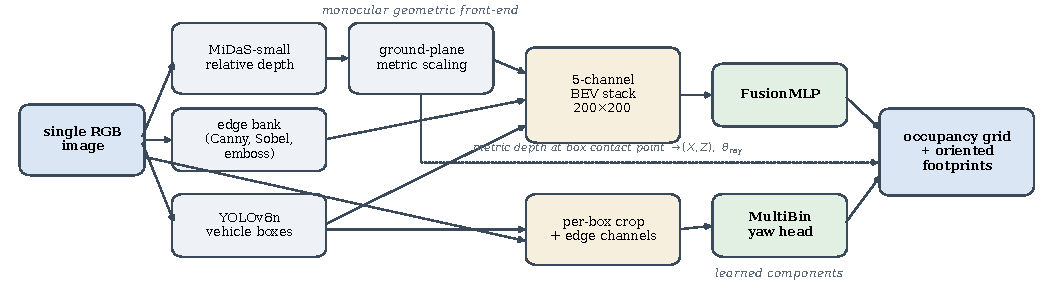
\includegraphics[width=\textwidth]{figs/fig1_pipeline.pdf}
  \caption{The pipeline. A single uncalibrated RGB image is turned into a five-channel BEV feature stack by three parallel branches; a learned per-cell fusion produces the occupancy grid, and a MultiBin head over detector crops produces vehicle orientation, which is composed with the ray angle from the same depth map to place oriented footprints on the grid.}
  \label{fig:pipeline}
\end{figure*}

\subsection{Metric depth from an uncalibrated image}\label{sec:depth}

We estimate relative inverse depth $d(u,v)$ with MiDaS-small~\cite{ranftl2022midas}, chosen over the stronger DPT-Hybrid~\cite{ranftl2021dpt} for inference cost; Section~\ref{sec:backbone} quantifies what that choice costs.

Since no calibration file exists, we assume a pinhole camera with $f_x = f_y = 0.85W$ and the principal point at the image centre, where $W$ is the image width. This corresponds to a horizontal field of view of roughly $61^\circ$, typical of phone and dashcam optics.

To obtain metric depth we assume that the image band between $0.75H$ and $0.95H$ is flat ground at a fixed camera height $h = 1.5$\,m. For a forward-facing camera with no pitch, the ray through row $v$ meets that ground plane at
\begin{equation}
Z_{\text{ground}}(v) = \frac{h\,f_y}{v - c_y}, \qquad v > c_y,
\end{equation}
and treating the network output as inverse depth up to a single scale $s$, $Z(u,v) = s/d(u,v)$, we solve for $s$ by matching the two over the ground band:
\begin{equation}\label{eq:scale}
s = \operatorname{median}_v \big( Z_{\text{ground}}(v)\cdot \bar{d}(v) \big),
\end{equation}
where $\bar{d}(v)$ is the row-averaged relative depth. Metric depth is then clipped to $[0.5, 80]$\,m to discard the numerically unstable region near the horizon.

Equation~\eqref{eq:scale} carries every metric assumption in the system, and it is worth being blunt about its weaknesses. It fits a scale but no shift, whereas mixed-dataset relative depth is only defined up to an affine transform of disparity; it assumes zero camera pitch and a flat, visible, unoccluded ground band; and $h = 1.5$\,m is a guess. The consequences are visible in our results and revisited in Section~\ref{sec:limits}.

\subsection{BEV grid and feature channels}\label{sec:grid}

The BEV grid covers $Z \in [0, 40]$\,m forward and $X \in [-20, 20]$\,m laterally at 0.2\,m per cell, giving a 200$\times$200 array. Every pixel with valid depth is back-projected, $X = (u - c_x)Z/f_x$, and accumulated into cell $(\lfloor Z/\delta\rfloor, \lfloor (X+20)/\delta \rfloor)$ with $\delta = 0.2$\,m. We accumulate the count $n$, the depth sum, and the depth sum-of-squares per cell, from which five channels are formed:
\begin{enumerate}
\item \textbf{Density}: $n/\max n$, normalised per image.
\item \textbf{Edge confidence}: a weighted combination of Canny, normalised Sobel magnitude, and normalised emboss response (0.4/0.4/0.2), computed in the image plane and projected into BEV by averaging the values of all pixels falling in a cell.
\item \textbf{Detector confidence}: for every YOLOv8n~\cite{jocher2023yolov8} detection of a COCO~\cite{lin2014coco} vehicle class (car, motorcycle, bus, truck) above confidence 0.35, the depth at the box's bottom-centre pixel places the vehicle in BEV, and a 3$\times$3 neighbourhood is set to the detection confidence by maximum.
\item[4--5.] \textbf{Depth mean and variance} per cell, computed from the accumulated sums.
\end{enumerate}
Cells receiving no projected point have all five channels equal to zero. We refer to the set of cells with $n \geq 1$ as the \emph{geometric support} of an image; it is an upper bound on what any function of these channels can mark occupied, and it is the reference against which we measure transfer behaviour in Section~\ref{sec:transfer}.

\subsection{Pseudo-labels and learned fusion}\label{sec:fusion}

\paragraph{Supervision.} On KITTI's \texttt{val\_\allowbreak selection\_\allowbreak cropped} split, which provides LiDAR-derived ground-truth depth and per-frame intrinsics~\cite{uhrig2017sparsity}, we replace the estimated depth of Section~\ref{sec:depth} with the ground-truth depth map and the assumed intrinsics with the real ones, run the identical accumulation, and define a cell as occupied when it receives at least three projected LiDAR points. This yields \rev{1{,}000 (input, label) pairs. We use two splits: a random 850/150 split (15\% held out), and a 726/274 split that holds out whole drives so that near-duplicate frames from one drive never straddle the split.}

\begin{revised}
\paragraph{Two input regimes.} The labels are always the ones just described. The \emph{inputs} to the fusion models are built in one of two ways. In the \emph{oracle} regime they come from the same ground-truth depth and real intrinsics as the labels; it is retained as a reference. In the \emph{front-end} regime they come from the pipeline as deployed: estimated depth (MiDaS-small with Equation~\eqref{eq:scale}, or Depth Anything V2) and the assumed intrinsics of Section~\ref{sec:depth}. Only the front-end regime reflects the uncalibrated setting the paper is about.
\end{revised}

\paragraph{FusionMLP.} A three-layer network of 1$\times$1 convolutions ($5 \rightarrow 16 \rightarrow 16 \rightarrow 1$, ReLU) applied identically to every cell. It is a per-cell MLP by construction: it can learn an arbitrary nonlinear recalibration of the five channels but has no access to spatial context. It has 421 parameters.

\paragraph{U-Net + PatchGAN.} A four-level U-Net generator (base width 32, skip connections, input reflection-padded to a multiple of 16) trained against a three-block PatchGAN discriminator~\cite{isola2017pix2pix} that sees the input stack concatenated with the occupancy map. The generator loss is $\mathcal{L}_G = \mathcal{L}_{\text{BCE}} + \lambda_{\text{adv}}\mathcal{L}_{\text{adv}}$ with $\lambda_{\text{adv}} = 0.1$, deliberately small: the adversarial term is intended to discourage speckle, not to dominate reconstruction.

Both models are trained with positive-weighted binary cross-entropy, the per-batch positive weight $n_{\text{neg}}/n_{\text{pos}}$ capped at 50 to avoid instability on near-empty grids. We use Adam, learning rate $10^{-3}$ for the MLP (60 epochs) and $2\times10^{-4}$, $\beta_1 = 0.5$ for the GAN (80 epochs), batch size 8, and restore the best-validation-IoU checkpoint rather than the final epoch.

\begin{revised}
\paragraph{Reference baselines.} Since no published single-image BEV method operates without intrinsics, we add two references that bound any method that thresholds the density channel. \emph{Density (isotonic)} fits a monotone isotonic regression~\cite{zadrozny2002isotonic} from the density channel to the label on the training split, i.e.\ the best possible global recalibration of density alone. \emph{Oracle threshold} chooses, for each test image separately, the density threshold that maximises that image's IoU using its label; no deployable density-only method can exceed it.
\end{revised}

\paragraph{Threshold selection \rev{and metrics}.} The hand-tuned score is a weighted sum of per-image-normalised channels and is not calibrated to any particular cutoff, whereas the trained models emit probabilities. Comparing all three at a fixed 0.5 would therefore be a comparison of calibration rather than of content. We report both a fixed 0.5 operating point and the best-F1 operating point found by sweeping thresholds in $[0.05, 0.95]$, and treat the latter as the fair comparison. \rev{We additionally report threshold-free average precision (AP), 95\% bootstrap confidence intervals over test images~\cite{efron1993bootstrap}, and means over three training seeds.}

\subsection{4-DoF vehicle pose}\label{sec:posemethod}

For each detected vehicle we estimate a ground-plane pose $(X, Z, \theta)$ and draw a fixed-template footprint of $4.5 \times 1.8$\,m.

\paragraph{Orientation head.} Following MultiBin~\cite{mousavian2017multibin}, we predict the observation angle $\alpha$ (the vehicle's orientation relative to the ray through it) as a classification over angular bins plus a within-bin $(\cos,\sin)$ residual. We use a simplified single-target-bin encoding with $N_{\text{bins}} = 2$\rev{, so the bin classifier makes a front/back decision}; the consequences of that simplification are analysed in Section~\ref{sec:pose}. The backbone is a ResNet-18~\cite{he2016resnet} whose first convolution is widened from three to six input channels: RGB plus the same Canny, Sobel, and emboss maps used in the fusion stack, here kept as \emph{separate} channels so the network can learn which edge operator carries orientation information rather than inheriting the fixed weighting of Section~\ref{sec:grid}. The three new channels are initialised with the per-output-channel mean of the pretrained RGB weights. Two linear heads produce bin logits and $\ell_2$-normalised residuals. Training uses KITTI 3D object detection labels, restricted to Car and Van instances with truncation $\leq 0.5$, occlusion level $\leq 2$, and box side $\geq 10$\,px, with cross-entropy on the bin and smooth-$\ell_1$ on the target bin's residual.

\paragraph{Global yaw and footprint.} Given the detector box, we take the depth $Z$ at its bottom-centre pixel, recover $X = (u_{bc} - c_x)Z/f_x$, and compute the ray angle $\theta_{\text{ray}} = \arctan(X/Z)$. The global yaw is
\begin{equation}\label{eq:yaw}
\theta = \operatorname{wrap}\big(\alpha + \theta_{\text{ray}}\big),
\end{equation}
wrapped to $[-\pi, \pi]$. The footprint corners are the canonical rectangle rotated by $\theta$ and translated to $(X,Z)$, then rasterised into grid coordinates. We stress that translation here is the same back-projection used to place the detector-confidence channel, not the closed-form 2D--3D box-edge fit of Mousavian et al.; this keeps the footprint consistent with the occupancy map beneath it, at the price of inheriting the depth error of Equation~\eqref{eq:scale}.

%% ------------------------------------------------------------------
\section{Experiments}

\subsection{Setup}

\paragraph{Source domain.} KITTI~\cite{geiger2012kitti} supplies both the occupancy pseudo-labels (\texttt{val\_\allowbreak selection\_\allowbreak cropped}, with per-frame intrinsics) and the orientation supervision (3D object detection training split). \rev{Occupancy uses the random 850/150 and the drive-held-out 726/274 splits of Section~\ref{sec:fusion}; orientation uses a random split with 15\% held out.}

\paragraph{Target domain.} Our transfer set is a subset of crowd-sourced street-level imagery~\cite{neuhold2017mapillary} at 4096$\times$3072 resolution. To avoid cherry-picking, we select the evaluation images by a fixed protocol: embed every candidate with CLIP ViT-B/32~\cite{radford2021clip}, run $k$-means with $k = 40$ (seed 42), and take the image nearest each centroid. This yields 40 images spanning the visual diversity of the pool rather than 40 images we liked. All in-the-wild results below are on exactly this set.

\paragraph{Reproducibility.} All experiments run on a single GPU. Splits and clustering use seed 42; \rev{fusion models are trained with three seeds where a mean and standard deviation are reported, and with seed 42 otherwise.} Checkpoints, the 40-image selection list, the per-image occupancy grids, and the pose records are released with the paper.

\subsection{How much does the depth backbone cost?}\label{sec:backbone}

Before evaluating fusion, we quantify the quality of the depth on which everything rests. Table~\ref{tab:depth} compares MiDaS-small against DPT-Hybrid on KITTI and Make3D~\cite{saxena2009make3d} with per-image least-squares scale-and-shift alignment, the standard protocol for relative-depth models.

\begin{table}[t]
\caption{Depth backbone quality under per-image scale-and-shift alignment. KITTI: 100 images from \texttt{val\_\allowbreak selection\_\allowbreak cropped}. Make3D: 425 pairs. Lower AbsRel is better; higher $\delta_1$ is better.}
\label{tab:depth}
\begin{tabular}{llcc}
\toprule
Dataset & Backbone & AbsRel $\downarrow$ & $\delta_1$ $\uparrow$ \\
\midrule
KITTI & MiDaS-small & 0.273 & 0.551 \\
KITTI & DPT-Hybrid & 0.121 & 0.880 \\
Make3D & MiDaS-small & 0.292 & --- \\
Make3D & DPT-Hybrid & 0.272 & --- \\
\bottomrule
\end{tabular}
\end{table}

The gap is large on KITTI and small on Make3D, which is itself informative: on driving-like scenes the stronger backbone is substantially better, while on the more heterogeneous Make3D imagery the two converge. Since our target domain is closer to Make3D in heterogeneity than to KITTI, the choice of the cheaper backbone is defensible --- but every metric result that follows should be read as conditioned on a depth estimate whose relative error on driving scenes is around 27\%.

\subsection{Occupancy fusion on oracle inputs}\label{sec:oracle}

\begin{table}[t]
\caption{\rev{Occupancy fusion on \emph{oracle} inputs (ground-truth depth and intrinsics), held-out KITTI split.} @0.5 is a fixed threshold; @best sweeps the threshold and reports the best-F1 operating point. The hand-tuned score is not calibrated to any cutoff, so @best is the fair column. \rev{@0.5 is seed 42. FusionMLP @best is the mean $\pm$ s.d.\ over three seeds (seed 42 alone: 0.822 at $t{=}0.85$); other entries are single runs.}}
\label{tab:oracle}
\begin{tabular}{lcc}
\toprule
Method & IoU@0.5 & IoU@best \\
\midrule
Hand-tuned (0.5/0.2/0.3) & 0.000 & 0.251 \\
\rev{Density (isotonic)} & \rev{---} & \rev{0.812} \\
U-Net + PatchGAN & 0.722 & \rev{0.724} \\
FusionMLP & 0.694 & \rev{$0.805 \pm 0.018$} \\
\bottomrule
\end{tabular}
\end{table}

Table~\ref{tab:oracle} reports all fusion strategies on the identical held-out split against the identical pseudo-labels\rev{, with ground-truth depth and intrinsics as inputs. This is not the uncalibrated setting, and we report it as an oracle reference beside the front-end results of Section~\ref{sec:frontend}.}

\rev{Three} observations. First, the hand-tuned weighting is not merely worse, it is catastrophically miscalibrated at a 0.5 cutoff: because the density channel is normalised by its per-image maximum, almost no cell ever reaches 0.5, and IoU collapses to $3\times10^{-4}$. Even at its own best threshold of 0.05 it reaches only 0.251 IoU. This is the clearest possible evidence that a hand-chosen weighted sum over heterogeneously normalised channels has no meaningful operating point.

Second, the per-cell MLP outperforms the spatially aware U-Net at the fair operating point (\rev{$0.805\pm0.018$} versus \rev{0.724} IoU), despite having 421 parameters against roughly $10^6$. We read this as a statement about the task rather than about architectures: with the label defined cell-wise from projected point counts, spatial context contributes little \rev{when the inputs already carry the true geometry}.

\begin{revised}
Third, and decisively, an isotonic recalibration of the density channel alone reaches 0.812 IoU, and FusionMLP does not differ from it in AP ($\Delta\text{AP} = -0.004$, 95\% CI $[-0.008, 0.001]$). The whole gain from 0.251 to 0.805 is therefore calibration. This confirms experimentally what is also true structurally: the pseudo-label is $\mathbb{I}[n \geq 3]$ while the first input channel is $n/\max n$, so on oracle inputs the label is a thresholded, monotone function of one input up to the per-image normalisation. Learning the fusion recovers a calibrated occupancy decision that a hand-tuned weighted sum destroys --- a real and useful finding, as Section~\ref{sec:transfer} shows, but not evidence that the auxiliary channels contribute new structure. Whether they do can only be asked on front-end inputs, which we turn to next.
\end{revised}

\begin{revised}
\subsection{Occupancy fusion without ground-truth calibration}\label{sec:frontend}

\begin{table*}[t]
\caption{Occupancy fusion on \emph{front-end} inputs: estimated depth and assumed intrinsics ($f{=}0.85W$, central principal point, $h{=}1.5$\,m), with the same KITTI labels as Table~\ref{tab:oracle}. Entries are IoU@best\,/\,AP; the oracle threshold is per image and reported as IoU only. U-Net is the mean of three seeds ($\pm0.002$ for MiDaS-small).}
\label{tab:frontend}
\begin{tabular}{lccccc}
\toprule
Depth source (assumed intrinsics) & Hand-tuned & Density (isotonic) & Oracle threshold & FusionMLP & U-Net + PatchGAN \\
\midrule
MiDaS-small + Eq.~\eqref{eq:scale} (ours) & 0.101\,/\,0.171 & 0.197\,/\,0.213 & 0.208 & 0.245\,/\,0.299 & 0.419\,/\,0.610 \\
Depth Anything V2$^\dagger$ & 0.127\,/\,0.243 & 0.281\,/\,0.338 & 0.295 & 0.381\,/\,0.502 & 0.461\,/\,0.666 \\
\bottomrule
\end{tabular}

\vspace{2pt}
\raggedright\small $^\dagger$Outdoor metric model, fine-tuned on Virtual KITTI 2~\cite{cabon2020vkitti2}; it therefore has a domain advantage on KITTI.
\end{table*}

Table~\ref{tab:frontend} repeats the comparison with the inputs the pipeline actually produces. As an external reference we substitute the state-of-the-art off-the-shelf metric depth model, Depth Anything V2~\cite{yang2024depthanythingv2}, for our depth stage, keeping the same assumed intrinsics. With no ground-truth calibration anywhere, the pipeline reaches 0.461 IoU (0.419 with our MiDaS-small front-end) against 0.127 (0.101) for hand-tuned fusion on the same inputs. Unlike the oracle regime, both learned models now exceed both density references: FusionMLP improves on isotonic density by $+0.087$ AP (95\% CI $[0.075, 0.099]$) and even on the per-image oracle threshold (0.245 versus 0.208 IoU), so on front-end inputs the fusion is doing more than a global recalibration of density. These conclusions also hold on the drive-held-out 726/274 split, with threshold-free AP, bootstrap confidence intervals, and three seeds.

\begin{table}[t]
\caption{Where the oracle-to-front-end drop comes from (IoU@best, same labels). Rows replace one oracle input at a time with its front-end counterpart; GT = ground truth.}
\label{tab:decomp}
\setlength{\tabcolsep}{4pt}
\begin{tabular}{llccc}
\toprule
Depth & Intrinsics & Density (iso.) & FusionMLP & U-Net \\
\midrule
GT & GT & 0.812 & 0.805 & 0.724 \\
GT & assumed & 0.34 & 0.379 & 0.581 \\
MiDaS-small & GT & 0.29 & 0.33 & --- \\
MiDaS-small & assumed & 0.197 & 0.245 & 0.419 \\
\bottomrule
\end{tabular}
\end{table}

Table~\ref{tab:decomp} decomposes the drop from the oracle reference. Replacing the intrinsics alone costs more than replacing the depth alone (0.34\,/\,0.38 versus 0.29\,/\,0.33 for density-only\,/\,FusionMLP), and the two errors compound to 0.20\,/\,0.25 for the full front-end. The assumed intrinsics are thus as large a source of error as the cheap depth network --- consistent with Section~\ref{sec:limits}, where focal-length error scales lateral position linearly. Note also that with exact depth but assumed intrinsics the U-Net reaches 0.581 against 0.379 for FusionMLP; Section~\ref{sec:where} examines why.

\subsection{Where does the front-end gain come from?}\label{sec:where}

\paragraph{FusionMLP: a range-dependent recalibration.} Removing the depth-mean channel drops FusionMLP on front-end inputs to exactly the density-only value (0.197 IoU); removing any other single channel changes IoU by at most 0.0003. Because all points falling in a cell share its 0.2\,m range bin, the depth-mean channel encodes range. The per-cell model's advantage over density is therefore a range-dependent recalibration of density --- a more useful calibration than a global one, but still a calibration rather than evidence from the edge or detector channels.

\paragraph{U-Net: partly calibration to the training camera.} A spatial model trained on a single camera could learn to undo that camera's specific mismatch with the assumed intrinsics. We tested this by changing the assumed focal length to 0.70, 0.85, and 1.00$W$ (the true KITTI value is $\approx 0.59W$) independently at training and test time. FusionMLP depends only on the test-time assumption and is identical whichever assumption it was trained on. U-Nets trained and tested on the same assumption all reach 0.41--0.42: they absorb the mismatch. A train/test mismatch costs the U-Net 0.03--0.10 IoU, yet it stays above FusionMLP (0.32--0.39). The U-Net's front-end gain is therefore part single-camera calibration and part spatial context, and we do not present it as calibration-free. Removing the adversarial loss leaves the U-Net unchanged (0.421 versus 0.417 IoU); the term only makes 0.5 the optimal threshold, which is why its @0.5 and @best values coincide in Table~\ref{tab:oracle}.

\paragraph{Choice for transfer.} For the in-the-wild images of Section~\ref{sec:transfer}, whose cameras are unknown and differ from KITTI's, we keep FusionMLP: its behaviour depends only on the test-time assumption, whereas part of the U-Net's advantage is tied to the training camera and cannot be assumed to transfer.
\end{revised}

\subsection{Transfer to uncalibrated in-the-wild imagery}\label{sec:transfer}

On the 40-image target set there is no ground truth of any kind, so accuracy cannot be reported and we do not report it. What can be measured is whether the occupancy decision remains geometrically sensible: whether it covers the cells that actually received projected points, whether it invents structure outside that support, and whether the resulting map is spatially coherent or speckled. Table~\ref{tab:transfer} reports these statistics over all $40 \times 200 \times 200 = 1.6$M cells.

\begin{table}[t]
\caption{Transfer behaviour on 40 diversity-sampled in-the-wild images. Each method is evaluated at \rev{a fixed operating threshold} (0.05 hand-tuned, 0.5 FusionMLP). Support recovery is the fraction of geometrically supported cells marked occupied; support precision is the fraction of occupied cells that lie inside the support; speckle is the fraction of occupied cells with no 4-connected occupied neighbour.}
\label{tab:transfer}
\begin{tabular}{lcc}
\toprule
Statistic & Hand-tuned & FusionMLP \\
\midrule
Occupied cells (\%) & 6.4 & 34.4 \\
Support recovery (\%) & 14.0 & 75.2 \\
Support precision (\%) & 100.0 & 100.0 \\
Speckle (\%) & 23.3 & 2.3 \\
Connected components / image & 855 & 409 \\
Mean score & 0.013 & 0.316 \\
\midrule
\multicolumn{3}{l}{Geometric support: 45.7\% of cells} \\
\multicolumn{3}{l}{Pearson correlation of the two scores: $0.546 \pm 0.073$} \\
\bottomrule
\end{tabular}
\end{table}

The pattern is consistent with the calibration reading of Section\rev{s~\ref{sec:oracle}--\ref{sec:where}}. Both methods are perfectly precise with respect to the geometric support --- neither ever marks a cell occupied that received no projected point, which is expected given that all five channels vanish there, but is worth confirming rather than assuming. Where they differ is recall: the hand-tuned score, even at its most permissive useful threshold, marks only 14.0\% of the supported cells, discarding the large majority of the geometric evidence the front-end produced. The learned fusion recovers 75.2\%. It is also an order of magnitude less speckled (2.3\% versus 23.3\% isolated cells) and produces half as many connected components, meaning the surviving structure is contiguous rather than scattered. The moderate per-image correlation between the two scores (0.546) confirms that the learned model is not simply a rescaling of the hand-tuned one.

Figure~\ref{fig:stats}(a) shows where the difference lies in range. The hand-tuned score is flat at 5--8\% occupancy across the entire 40\,m, tracking neither the geometry nor the density of evidence. The learned fusion follows the geometric support closely out to about 25\,m and then falls away, which is the desired behaviour: beyond that range the projected points are sparse, the depth estimate is least reliable (the ground-plane fit of Equation~\eqref{eq:scale} degrades near the horizon), and the model correctly becomes less confident rather than filling the far field.

Figure~\ref{fig:scenes} shows three scenes qualitatively. The visible radial striping in the far field of the learned maps is a genuine artefact and not a rendering effect: it is the signature of the missing affine shift in Equation~\eqref{eq:scale}, which distorts the mapping from disparity to metric depth most severely where disparity is small.

\begin{figure*}[t]
  \centering
  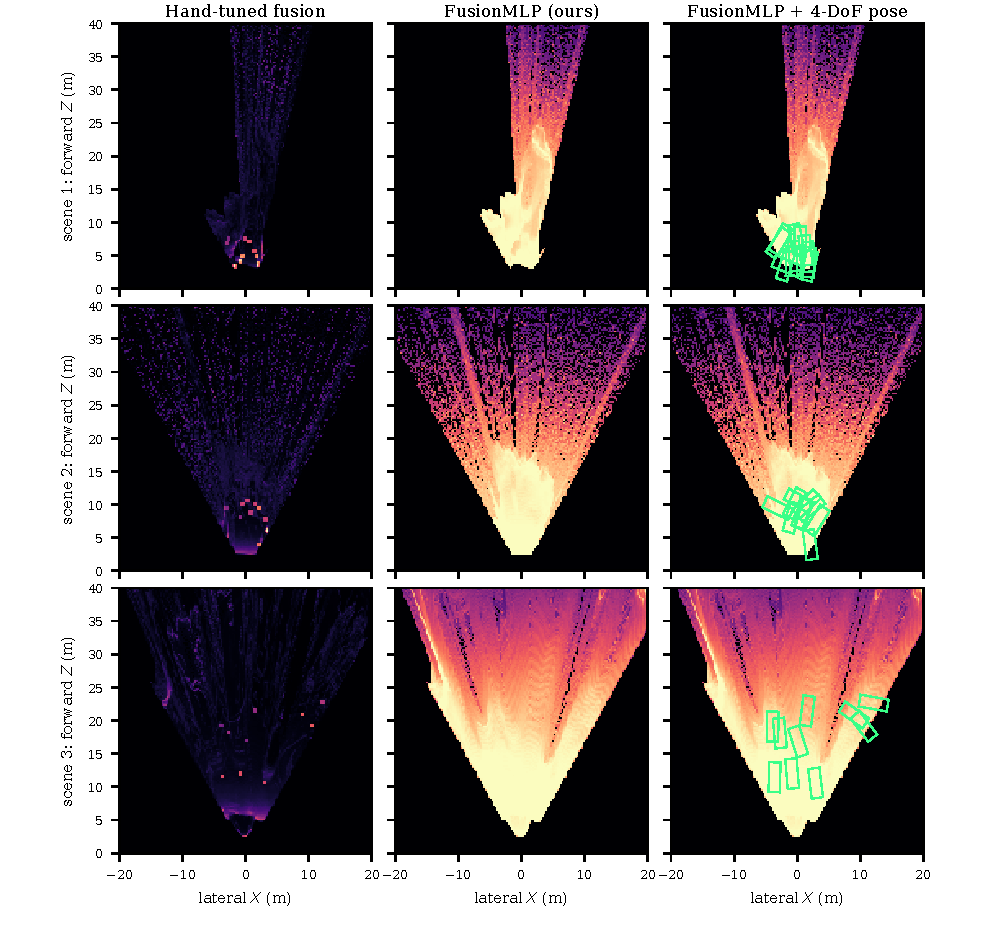
\includegraphics[width=0.62\textwidth]{figs/fig2_scenes.pdf}
  \caption{Three in-the-wild scenes (ego-vehicle at the bottom centre of each panel). Left: hand-tuned fusion, shown at a 2.5$\times$ boosted colour scale so that anything is visible at all. Centre: learned per-cell fusion. Right: the same map with 4-DoF oriented vehicle footprints. The radial striping at long range is the affine-shift artefact discussed in Section~\ref{sec:limits}.}
  \label{fig:scenes}
\end{figure*}

\begin{figure*}[t]
  \centering
  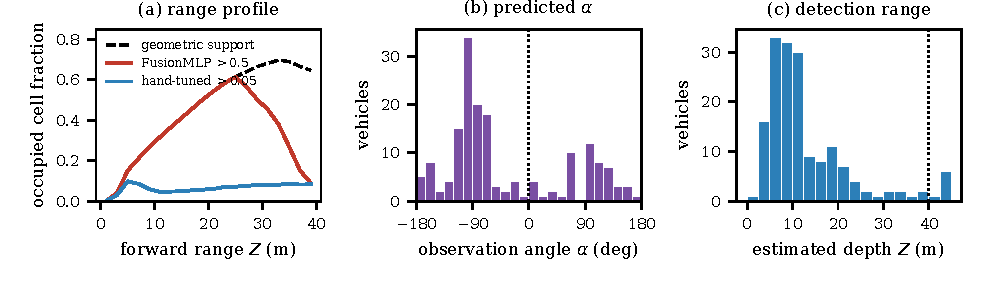
\includegraphics[width=0.92\textwidth]{figs/fig3_stats.pdf}
  \caption{(a) Fraction of occupied cells against forward range, averaged over the 40 in-the-wild images; the dashed curve is the geometric support. (b) Distribution of predicted observation angle $\alpha$ over 168 vehicles; dotted lines mark the two MultiBin bin centres. (c) Estimated depth of the same vehicles; the dotted line marks the grid's 40\,m range limit.}
  \label{fig:stats}
\end{figure*}

\subsection{4-DoF pose integration}\label{sec:pose}

The orientation head reaches a held-out bin accuracy of \rev{97.85\%} and a mean angular error of \rev{$3.77^\circ$} on the KITTI split, trained on \rev{27{,}965 filtered Car/Van instances (4{,}194 held out). With two bins, bin accuracy measures only a front/back decision, so it is a coarse indicator of orientation quality.}

Applied to the 40 in-the-wild images, the pose stage produces 168 vehicle poses; 35 of the 40 images contain at least one, with a median of 4 and a maximum of 12. The detected class mix is 150 cars, 17 trucks, and 1 bus, at a mean detector confidence of 0.637. Estimated depths (Figure~\ref{fig:stats}(c)) have a median of 10.1\,m and an interquartile range of 7.1--16.6\,m, and 95.8\% fall inside the grid's 40\,m range; the ray angles are correspondingly modest, $|\theta_{\text{ray}}| \leq 29.8^\circ$, so Equation~\eqref{eq:yaw} is dominated by the learned term.

The orientation distribution (Figure~\ref{fig:stats}(b)) is where the interesting failure lies. Of the 168 predictions, 78.6\% fall in the near-perpendicular band $45^\circ \leq |\alpha| \leq 135^\circ$, and 56.0\% in the single quadrant $[-135^\circ, -45^\circ]$. Only 8.3\% are predicted as facing away from the camera and 13.1\% as facing towards it. That is not a plausible distribution for street-level photography, which is dominated by vehicles ahead of and receding from the camera, and it is not attributable to the scenes: it is what a two-bin MultiBin head produces when the bin classifier is weakly informative \rev{on the target domain} and the residual regression, which can express at most a half-turn correction from each bin centre, settles near the midpoint between them. We regard $N_{\text{bins}} = 2$ as the identified defect of this stage; the standard MultiBin configuration uses overlapping bins with $N \geq 4$, and the residual encoding should be revisited alongside it.

We deliberately do not report an orientation accuracy figure on the target domain. There is no orientation ground truth for these images, and the model's own predictions cannot grade themselves. We have extracted all 168 vehicle crops and prepared a coarse four-way facing-direction labelling protocol (away, toward, left, right) with a zero-shot versus few-shot comparison harness; completing that annotation is the immediate next step and is not claimed as a result here.

\subsection{A negative result on VLM-based evaluation}\label{sec:vlm}

Faced with a target domain that has no ground truth, we attempted to replace human judgement with a vision-language model. A Qwen2-VL-2B-Instruct judge~\cite{wang2024qwen2vl} was shown each input photograph alongside its BEV map and asked to score three axes from 1 to 5: road-boundary visibility, object placement plausibility, and absence of geometric artefacts. The same 40 maps were rated independently by a human using the same rubric. Table~\ref{tab:vlm} summarises the outcome.

\begin{table}[t]
\caption{VLM judge versus a human rater on the same 40 BEV maps and rubric. $\kappa_{\text{lin}}$ is linear-weighted Cohen's kappa~\cite{cohen1968kappa}. The artefact axis received a constant score of 5 from the judge, making both $\kappa$ and $\rho$ undefined.}
\label{tab:vlm}
\begin{tabular}{lccc}
\toprule
Axis & VLM mean & $\kappa_{\text{lin}}$ & Spearman $\rho$ \\
\midrule
Road boundary & 4.65 & 0.042 & 0.324 ($p{=}0.044$) \\
Object placement & 4.68 & 0.022 & 0.234 ($p{=}0.151$) \\
Geometric artefacts & 5.00 (const.) & --- & --- \\
\bottomrule
\end{tabular}
\end{table}

The judge sits near the ceiling of every axis while the human rater sits near the floor, and the agreement is at chance: $\kappa_{\text{lin}}$ of 0.042 and 0.022. Only the road-boundary correlation reaches nominal significance, and would not survive correction for three comparisons.

A natural defence of the judge is that its scores are noisy. They are not. Rating the same 40 images twice at sampling temperature 0.7 produced $\kappa_{\text{lin}} = 1.000$ and a mean absolute difference of 0.000 on all three axes: the judge is perfectly deterministic despite stochastic decoding. It is not noisy, it is confidently and reproducibly measuring something other than what the rubric asks. We also compared the judge against two objective proxies computed directly from the maps --- a Hough-line road-boundary score and an isolated-cell artefact score --- and found a Spearman correlation of $-0.102$ ($p = 0.53$) on the boundary axis.

We report this because the failure is easy to miss: a judge that always answers 4.7 produces a table that looks like a strong result. The lesson we draw is that for a geometric task with no ground truth, a small VLM judge should be validated against human ratings before use, not instead of them, and that self-consistency is not evidence of validity. Our own use of a single human rater is itself a limitation --- with $n = 1$ we can measure disagreement with the judge but cannot establish the human ceiling --- which is why we base the quantitative claims of Section~\ref{sec:transfer} on geometric statistics instead.

%% ------------------------------------------------------------------
\section{Limitations}\label{sec:limits}

We collect the caveats already raised, together with several that have not been.

\paragraph{The metric scale is an assumption, not a measurement.} Equation~\eqref{eq:scale} fits a scale but not the shift term that mixed-dataset relative depth also requires, assumes zero pitch, assumes the lower image band is flat unoccluded ground, and assumes $h = 1.5$\,m. Each failure of these assumptions is a global distortion of the map. The radial striping visible in Figure~\ref{fig:scenes} is the shift term's signature.

\paragraph{The assumed intrinsics are a heuristic.} $f_x = f_y = 0.85W$ with a central principal point is a plausible average across consumer optics, not the camera that took any particular photograph. Focal-length error scales lateral position linearly\rev{; Table~\ref{tab:decomp} shows it costs as much IoU as the depth network does}.

\paragraph{\rev{The random KITTI split is optimistic.}} Frames in \texttt{val\_\allowbreak selection\_\allowbreak cropped} are drawn from continuous drives, so a random 15\% split places near-duplicate frames on both sides. \rev{We therefore also report the drive-held-out split, on which our conclusions hold; absolute numbers on the random split should still be read as upper bounds.}

\paragraph{The pseudo-label is a function of an input channel.} As \rev{shown experimentally} in Section~\ref{sec:oracle}, this bounds what the oracle-input fusion comparison can establish\rev{; front-end inputs (Section~\ref{sec:frontend}) break that dependence only partially, since the per-cell gain is itself a recalibration (Section~\ref{sec:where})}.

\begin{revised}
\paragraph{The U-Net gain is not calibration-free.} Part of the U-Net's front-end advantage comes from absorbing the training camera's mismatch with the assumed intrinsics (Section~\ref{sec:where}), and would not be expected to carry over to a camera with different optics without retraining.

\paragraph{No calibrated BEV method is compared.} MonoLayout, PON, and OFT require known intrinsics, so we compare against density-based reference bounds instead. Adding MonoLayout as a calibrated upper reference is a natural extension.
\end{revised}

\paragraph{The pose stage is coarse by construction.} Two MultiBin bins (Section~\ref{sec:pose}), a single $4.5 \times 1.8$\,m footprint template for every vehicle class including the detected trucks and bus, and translation from the ground-contact back-projection rather than the 2D--3D box-edge solve. Vehicles whose contact point is occluded receive a systematically over-estimated depth.

\paragraph{The evaluation set is small and unlabelled.} Forty images, selected by a fixed and reported protocol but still forty. All target-domain numbers are behavioural statistics, not accuracy.

\paragraph{Single frame, no temporal aggregation.} This is the setting we chose, but it means no multi-view constraint is available to correct any of the above.

%% ------------------------------------------------------------------
\section{Conclusion}

We have described a monocular BEV pipeline that requires nothing from its input beyond a single uncalibrated image, and we have tried to be precise about what its numbers mean. \rev{With ground-truth depth and intrinsics as inputs, replacing a hand-tuned weighted sum with learned fusion raises held-out IoU on KITTI pseudo-labels from 0.251 to 0.805, but an isotonic recalibration of density alone reaches 0.812: that gain is calibration. With the uncalibrated front-end, learned fusion reaches 0.419 IoU (0.461 with Depth Anything V2 depth) against 0.101 (0.127) for the hand-tuned sum, and exceeds every density-only reference; the per-cell gain is a range-dependent recalibration, and the U-Net's is part training-camera calibration and part spatial context.} On in-the-wild imagery, learned fusion raises geometric support recovery from 14.0\% to 75.2\% while cutting speckle by an order of magnitude. The attached 4-DoF pose stage integrates cleanly with the map it is drawn on, and its orientation predictions exhibit a diagnosable collapse towards the perpendicular configuration that we attribute to a two-bin MultiBin simplification.

The most transferable finding may be the negative one: on a geometric task with no ground truth, a small VLM judge was perfectly self-consistent, near-ceiling, and uncorrelated with a human rater, whereas geometric consistency statistics computed against the pipeline's own projected support proved informative. Immediate next steps are a proper affine (scale-and-shift) depth alignment, an overlapping-bin MultiBin head with $N \geq 4$, completion of the human facing-direction annotation over the 168 extracted vehicle crops, \rev{a calibrated reference such as MonoLayout,} and an occupancy supervision signal that is independent of the density channel.

\bibliographystyle{ACM-Reference-Format}
\bibliography{references}

\end{document}
